% REMEMBER: You must not plagiarise anything in your report. Be extremely careful.

\documentclass{l4proj}


%
% put any additional packages here
%
\usepackage{pgf-umlsd}
\usepackage{scalefnt}
\usepackage{tikz}
\usepackage{float}
\usepackage{pdfpages}
\usepackage{multirow}

\begin{document}


%==============================================================================
%% METADATA
\title{Where Is ECN Stripped On the Network?}
\author{Myles Lamb}
\date{March 26, 2021}

\maketitle

%==============================================================================
%% ABSTRACT
\begin{abstract}
    % Every abstract follows a similar pattern. Motivate; set aims; describe work; explain results.
    % \vskip 0.5em
    % ``XYZ is bad. This project investigated ABC to determine if it was better. 
    % ABC used XXX and YYY to implement ZZZ. This is particularly interesting as XXX and YYY have
    % never been used together. It was found that  
    % ABC was 20\% better than XYZ, though it caused rabies in half of subjects.''
    
    
 Explicit Congestion Notification (ECN) allows devices on the network to signal incipient congestion before congestive loss occurs. The middlebox internet has presented deployment issues for features such as ECN. In this paper we investigate where on the network ECN codepoints are altered by network devices. To achieve this we implement a new network analysis tool. We subsequently conduct a medium scale deployment of the tool to gather a variety of measurements from the network to ascertain whether; Differing ECT codepoints are treated consistently by network devices, whether the transport protocol in use influences the modification of ECT codepoints. 
    
    % This paper investigates where on the network ECT codepoints are removed by network devices, we investigate this through the production of a new network analysis tool, allowing for the observation of the modifications of packets on the network on the granularity of individual ECT code points.
\end{abstract}

%==============================================================================

% EDUCATION REUSE CONSENT FORM
% If you consent to your project being shown to future students for educational purposes
% then insert your name and the date below to  sign the education use form that appears in the front of the document. 
% You must explicitly give consent if you wish to do so.
% If you sign, your project may be included in the Hall of Fame if it scores particularly highly.
%
% Please note that you are under no obligation to sign 
% this declaration, but doing so would help future students.
%
\def\consentname {Myles Lamb} % your full name
\def\consentdate {26 March 2021} % the date you agree

\educationalconsent


%==============================================================================
\tableofcontents

%==============================================================================
%% Notes on formatting
%==============================================================================
% The first page, abstract and table of contents are numbered using Roman numerals and are not
% included in the page count. 
%
% From now on pages are numbered
% using Arabic numerals. Therefore, immediately after the first call to \chapter we need the call
% \pagenumbering{arabic} and this should be called once only in the document. 
%
% The first Chapter should then be on page 1. You are allowed 40 pages for a 40 credit project and 20 pages for a 
% 20 credit report. This includes everything numbered in Arabic numerals (excluding front matter) up
% to but excluding the appendices and bibliography.
%
% You must not alter text size (it is currently 10pt) or alter margins or spacing.
%
%
%==================================================================================================================================
%
% IMPORTANT
% The chapter headings here are **suggestions**. You don't have to follow this model if
% it doesn't fit your project. Every project should have an introduction and conclusion,
% however. 
%
%==================================================================================================================================


\chapter{Introduction}
\label{chap:introduction}

% reset page numbering. Don't remove this!
\pagenumbering{arabic} 

This chapter will motivate the development of a new network analysis tool to investigate the adoption of Explicit Congestion Notification (ECN). Additionally we investigate the frequency and location on the network where ECN expressions are altered by devices on the network path. Following chapters will go into detail, discussing various aspects of the project, such as the design and implementation of the network analysis tool and analysis of the results of a medium scale deployment of the previously developed tool.

ECN is an extension to the Internet Protocol (IP) and some higher level protocols such as Transmission Control Protocol (TCP) that allows devices on the network to signal incipient congestion and respond accordingly before packet loss due to network congestion occurs.

The deployment of ECN has been slowed due to issues relating to devices on the network dropping packets that attempt to utilise ECN, resetting connections that attempt to negoatiate ECN or remarking packets that indicate ECN capable transport (\cite{floyd_inappropriate_2002}), ultimately leading to a lack of faith in the technology. Whilst these issues have lessened in prevalence over time (\cite{trammell_enabling_2015}), there has been a renewed interest in the deployment of ECN through its integration with Quic, a new transport protocol operating over UDP (\cite{johansson_ecn_2017}), as well as the growing need to reduce queuing delay across modern networks, given the increasing prevalence of real time traffic, ultimately presenting the preservation of ECN markings across the network as critical for managing the continued development of the internet. To the best of our knowledge this paper presents first set of findings relating to the deployment of ECN within Quic. As well as presenting a new technical method for measuring on path removal of codepoints to TCP based hosts.



We present the aims of this paper as follows; We intend to investigate the overall adoption of ECN. Additionally we investigate where as well as how often devices on the network modify the expressions of ECN related marking on internet traffic. We also seek to discern whether choices in internet protocol version or transport layer substrate influence the remarking behaviour of devices on the network, incorporating new protocols that support ECN such as Quic. Lastly, we investigate whether the available ECT codepoints exhibit different behaviours from devices on the network. To achieve this we will; Devise a suitable experimental methodology to gather appropriate measurements from the network (Section \ref{chap:design}), Design and implement a network analysis tool supporting the goals of the experimental methodology (Section \ref{chap:design} and Section \ref{chap:implementation}), Evaluate the network analysis tool through a medium scale deployment across numerous geographically distributed hosts (Section \ref{chap:evaluation}).

\clearpage


%==================================================================================================================================
\chapter{Background}

This chapter discusses the fundamentals of ECN as a technology and presents the contributions of previous works. Identifying areas for elaboration in existing research.
\addtocontents{toc}{\protect\setcounter{tocdepth}{1}}

\section{Overview of ECN}

The traditional end to end approach to congestion control employed within transport protocols such as TCP results in end hosts inferring congestion on the network through signals such as packet loss. Whilst protocols such as TCP have managed well through the use of loss based congestion signals. With the advent of mobile computing and the internet of things, and implied wireless communication. It is not clear that loss based congestive signals are the most suitable.
ECN is a mechanism that allows for devices on the network to signal incipient congestion to end hosts before congestive loss occurs. This allows routers utilising Active Queue Management (ie. Random Early Detection) to mark packets when congestion is experienced. Receivers observing these markings inform the sender of their observation, allowing the sender to reduce their sending rate before a congestive loss occurs. This may potentially reduce negative aspects of loss based congestion signals such as, Head-of-line blocking for protocols that provide an in-order delivery service model such as TCP, or providing benefits to the quality of service for protocols that do not re-transmit lost packets such as Real-time Protocol (RTP).

ECN is implemented through 2 bits of the IPv4/IPv6 header. Namely, the 2 least significant bits of the Traffic Class byte, with the other 6 bits constituting the differentiated services codepoint (DSCP). These two bits of the IP header are used to signify whether a given transport is ECN capable, and whether congestion has been experienced on the network. We have four potential bit patterns using these bits, called ECT (ECN capable transport) codepoints. 00 = not ECN capable, 10 = ECT(0), 01 = ECT(1), 11 = CE (congestion experienced).

It may be noted that both ECT(0) and ECT(1) can be used to signal a given transport as ECN capable, and both are to be treated equivalently by devices on the network (\cite{floyd_addition_2001}). Furthermore if a device on the network does not leverage the ECN field, it is not to modify it. Historically, the bits that constitute the ECN field occupy the same space as the legacy ToS (Type of Service) byte, providing some insight into why ECN is removed on the network, with some older equipment on the network continuing to use ToS semantics and subsequently erroneously clearing the ECN field (\cite{kuhlewind_state_2013}).

Lastly, the CE codepoint is used by devices on the network to signal that congestion is incipient on a given node on the network. Routers that implement ECN related functionality typically employ an algorithm such as Random early detection (RED) to produce a probability of dropping packets in the future. If this is over a given threshold, the router will mark packets that indicate ECN capable transport with the congestion experienced codepoint, as a means to inform senders to reduce their sending rates.

\subsection{Historic use of ToS and its implications}

As previously mentioned, the bits in the IP header that constitute the ECN field did not always serve this purpose. Historically these bits constituted part of the Type of Service field, which served many related purposes over the years of its use. Originally presented in RFC 792 and further updated in RFC 1583 it was primarily used to identify the precedence of traffic as well as providing mechanisms to request specific treatment on the network such as, low latency, or high reliability. However the latter was seldom used outside of a few specific use case scenarios. Whilst efforts were made to ensure some level of compatibility between ToS and the later introduced DSCP (Differentiated Services Codepoint), such as maintaining the IP Precedence aspect of ToS. this could not be extended to ECN. The bits that constitute ECN where either unused as defined in RFC 792, or otherwise in RFC 1583 the rightmost bit was to always contain a value of zero. \cite{custura_exploring_2017} showed the existence of a number of devices on the internet that continue to use ToS based semantics, within a number of Autonomous Systems. exhibiting marking pathologies that are destructive towards ECN on the network.
% Discuss research concerning the %

\section{ECN within TCP}

When ECN is utilised with TCP, hosts must first negotiate its use at the beginning of the TCP connection, during the SYN-ACK exchange as part of TCP connection establishment. Utilising two, previously reserved bits of the TCP header. Namely the ECE (ECN Echo) and the CWR (Congestion window reduced) bits. Hosts may negotiate ECN through setting the ECE and CWR bits of the TCP header on the initiating SYN of the TCP handshake. If the receiving host also desires to use ECN, a SYN-ACK with the ECE bit set will be returned. Subsequent data segments sent during the connection should be marked with either ECT(0) or ECT(1) on the IP header to indicate ECN capable transport. Given when congestion is experienced on the network, and some device marks a given packet with the ECE codepoint. End hosts receiving a packet with the CE codepoint set, should respond by setting the ECE bit in the TCP header on the following segment sent during the connection. The sending host then indicates the receipt of a segment with ECE bit set, by setting the CWR bit in the TCP header of the following segment sent, as well as responding with respect to the congestion control algorithm in use as if packet loss had occurred, as summarised in figure \ref{fig:ecn_tcp}.



\begin{center}
    \begin{figure}[H]
            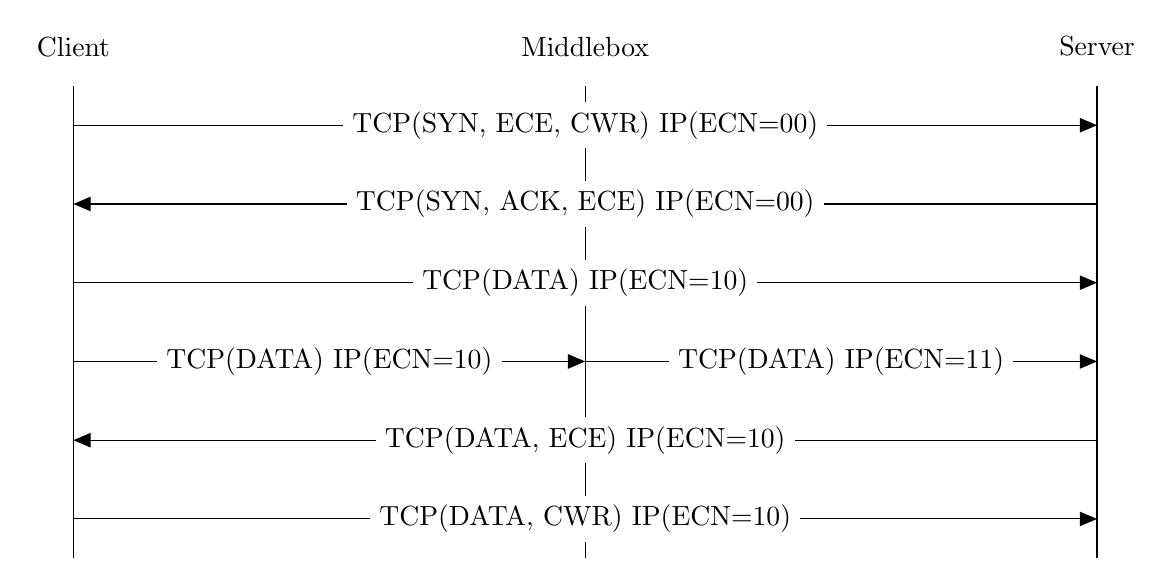
\begin{tikzpicture}
            
            \draw (0,0) -- (0, 6);
            \draw (6.5,0) -- (6.5, 6);
            \draw (13,0) -- (13, 6);
            \node at (0,6.5) {Client};
            \node at (6.5,6.5) {Middlebox};
            \node at (13,6.5) {Server};
            
            \draw [arrows={-triangle 45}]
            (0, 5.5) -- (13, 5.5) node [midway, fill=white, text centered]
            { TCP(SYN, ECE, CWR)  IP(ECN=00)};
            
            \draw [arrows={triangle 45-}]
            (0, 4.5) -- (13, 4.5) node [midway, fill=white, text centered]
            { TCP(SYN, ACK, ECE)  IP(ECN=00)};
            
            \draw [arrows={-triangle 45}]
            (0, 3.5) -- (13, 3.5) node [midway, fill=white, text centered]
            { TCP(DATA)  IP(ECN=10)};
            
            \draw [arrows={-triangle 45}]
            (0, 2.5) -- (6.5, 2.5) node [midway, fill=white, text centered]
            { TCP(DATA)  IP(ECN=10)};
            
            \draw [arrows={-triangle 45}]
            (6.5, 2.5) -- (13, 2.5) node [midway, fill=white, text centered]
            { TCP(DATA)  IP(ECN=11)};
            
            \draw [arrows={triangle 45-}]
            (0, 1.5) -- (13, 1.5) node [midway, fill=white, text centered]
            { TCP(DATA, ECE)  IP(ECN=10)};
            
            \draw [arrows={-triangle 45}]
            (0, 0.5) -- (13, 0.5) node [midway, fill=white, text centered]
            { TCP(DATA, CWR)  IP(ECN=10)};
            
            \end{tikzpicture}
        \caption{Diagrammatic representation of the operation of the ECN extension with TCP/IP with a congested link on the network. When a given device on the network experiences congestion, it remarks the ECN field of packets indicating ECN capable transport to the CE codepoint. TCP acks have been omitted for the sake of brevity.}
    \label{fig:ecn_tcp}
    \end{figure}
\end{center}
\section{ECN within UDP}

ECN is not directly used with UDP, the exact operation of ECN with UDP is deferred to the context of a higher layer protocol, such as RTP, or Quic, which utilise UDP as their transport substrate. In the following text, we discuss the operation of ECN within Quic, one of the protocols investigated in this paper. Quic introduced the notion of ECN support with an IETF draft \cite{johansson_ecn_2017} discussing its intended operation. Whilst Quic is still in development as a protocol (lacking an RFC ), we summarise the operation of UDP under Quic within the draft used within this paper (ietf-draft-29).

When ECN is utilised with Quic, the sender must first determine whether both the path and the end host support ECN marking. This is defined as whether ECT codepoints are not cleared on path, or packets setting ECT codepoints are dropped, as well as the end host being able to both view and set the ECN field on the IP header. This is achieved through sending early Quic packets marked with either ECT(0) or ECT(1). Assuming packets are received by the end host, the receivers response should contain an "ECN ACK Frame" containing counts of packets observed with ECT(0), ECT(1) or CE. Of which the sender must validate, to ensure that the path and host support ECN markings. Following this, the sender may continue to send ECT marked packets. If a sending host, receives an ECN Ack frame that increases the CE count. The sender is to reduce their congestion window, in a similar manner to as if a loss had occurred, similarly to ECN under TCP/IP.

\section{ICMP Quotations}
\label{sec:icmp}

Introduced in RFC 792, it is required for some ICMP responses to return the IP header and the first 8 bytes of associated data as a payload of the ICMP packet. In particular 'TTL exceeded in transit' ICMP responses, are required by the RFC to observe this behaviour. This allows for path level insight to the IP header, and specifically, insight into remarking behaviour of ECN codepoints from within the network. This mechanism is used extensively in the existing literature on network measurement. Additionally in RFC 1812 this behaviour is recommended to be extended to not just aspects of the packet header, but the entire IP packet, however \cite{noauthor_tracebox_nodate} notes that this behaviour is less commonly observed as to only being adopted by some major vendors of networking equipment. The general concept around using ICMP responses to gain path level insight into the network is through the implementation of a traceroute style utility. 

From a given end-host on the network, We begin through sending packets into the network with a Time to Live (TTL) of one. the TTL field of the IP header describes the lifetime of an IP packet. When an IP packet arrives at a router or other device on the network, it is to decrement the TTL of the packet by one. If the TTL reaches zero, the packet is to be dropped by the device, and an ICMP TTL exceeded response is to be sent in return. This response signifies that a packet was dropped on the network due to an expiring TTL, additionally as a payload we receive the contents of the IP header and at least the first 8 bytes of the originating packets contents, of which is known as an ICMP quotation. The sender in turn receives this ICMP response containing the packet and its contents as it was seen by the device. This can be inspected to determine whether particular modifications have occurred in transit, and roughly where on the network that this occurs. This process is then repeated for increasing TTL values such that the packet traverses further into the network. We typically stop this procedure when either the end host responds, or a given TTL value is reached. The process is summarised in figure \ref{fig:icmp}.

\begin{figure}[H]

\centering
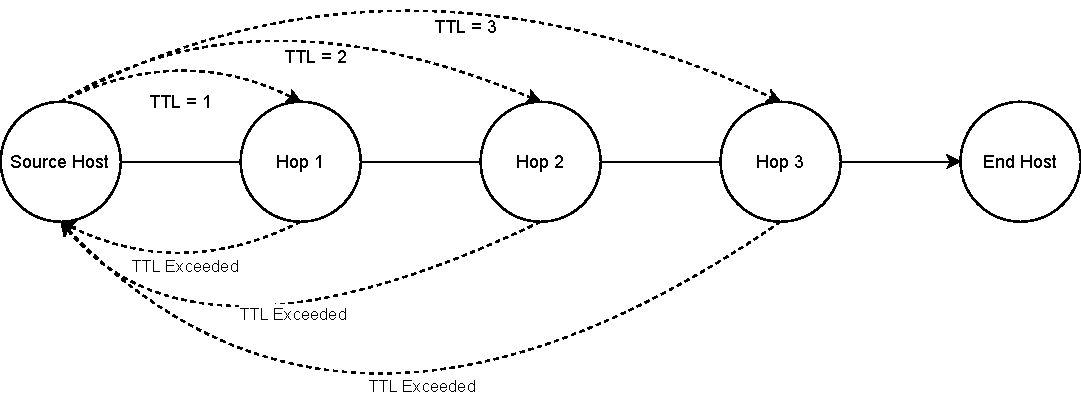
\includegraphics[width=14cm,keepaspectratio]{dissertation/images/icmp.pdf}
\caption{A diagrammatic representation of how ICMP quotations can be used to observe modifications to the IP header on the network path.}
\label{fig:icmp}
\end{figure}

\section{Previous Works}

There exists an extensive body of work on ECN measurement across the last two decades, in this subsection we present and evaluate previous contributions in the area.

\subsection{Measuring the state of ECN Readiness in clients and Servers}


There exists an extensive body of work on ECN measurement across the last two decades concerning the deployment of ECN within TCP. \cite{bauer_measuring_2011} measured the top one million web servers as ranked by the alexa top sites list, a collection of college and university based hosts and a collection of hosts intended for use with mobile devices. Measuring what fraction of hosts would negotiate ECN, additionally investigating whether middleboxes or routers on the network path were clearing ECT codepoints using an approach based on ICMP probes of the network as described in section \ref{sec:icmp}. From a collection of vantage points hosted in datacentres or university networks. The authors found that 94.8\% of hosts preserved the ECT codepoint across the network path. Additionally the authors observed many remarking behaviours for the ECN field, in some cases which transitions between several ECT codepoints before being set to zero value. The authors utilised a robust approach to identify a given interface that may be responsible for remarking the ECN codepoint, additionally attributing this behaviour to a particular AS, we see a particular bias to earlier in the network path, however this should be expected, as given when ECN codepoints are remarked subsequent parts of the network path are unable to be evaluated. This paper primarily used the CE codepoint in its network measurements, hence does not investigate the possibility of differential treatment of the codepoints on the network. Additionally, this paper was produced before the advent of the Quic network protocol hence it was not evaluated.


\subsection{Is ECN Usable With UDP}

Additional studies have also concerned themselves with the deployment of UDP based protocols incorporating ECN. \cite{mcquistin_is_2015} investigated in the broader sense whether ECN was usable with UDP, through the evaluation of 2,500 NTP pool servers. Revealing that ECN had a minor impact on the reachability of NTP servers. The authors briefly examined, where on the path ECT(0) codepoints were removed from packets, through implementing traceroutes to given hosts. Sending TTL limited packets with increasing hop limits until a response from the intended hosts is received. The generated ICMP TTL exceeded responses being collected in the process. The authors identified that in the majority of cases ECT(0) codepoints do traverse the network. Furthermore, when ECT codepoints are stripped from packets, this occurs distantly from the host, with the responsible device being located on an AS boundary. The authors did not use a directly comparable approach for that of TCP connections against the same host, although the core focus of the study was in evaluating the usability of UDP.

\subsection{Exploring DSCP Modification Pathologies in the Internet}

\cite{custura_exploring_2017} examined the wider traffic class byte. With a particular focus on the DSCP codepoint however the author discovers many different modification pathologies that in some cases effect ECN codepoints as well. In particular demonstrating a correlation between DSCP codepoint remarking and ECN remarking in many cases, suggesting that some routers erronously clear the ECN field as a consequence of continuing to use ToS semantics. However, this is not universal suggesting that not all ECN remarking behaviour is due to this observation. Furthermore the author investigates whether the transport protocol in use influences the DSCP modifications pathologies discussed in the paper. This analysis is not extended to the 3 non zero ECN codepoints individually, for which the modification pathologies slightly differ as shown in the paper.

\subsection{PathSpider}

There also exists a collection of existing tools tailored for network measurement. PathSpider is one of these tools, it is intended active measurement to reveal impairments on the network path. PathSpider allows for connections to a given host to be carried out in the format of an A/B test to reveal a given characteristic of the host or network path. For instance revealing whether a given connection to a host fails when ECN is negotiated. However for the purposes of this paper the default configurations of PathSpider were deemed insufficient. PathSpider treats the network at large as a black box. That is, PathSpider is sufficient at signalling when a given condition occurs, for example, whether a given TCP segement marked with ECE results in a CWR in response. However this signalling is not extended to where on the network path that the impairment occurs is located. Additionally newer protocols that are of interest, such as Quic do not have existing plugins supporting their analysis.

\subsection{Tracebox}

Tracebox is another network path transparency tool. Tracebox is viewed as a spiritual successor to the widely used traceroute tool allowing the user to identify the existence and behaviour of certain devices on the network such as NATs through evaluating ICMP responses as mentioned in section \ref{sec:icmp} against the source packet and identifying modifications. Whilst tracebox does feature a programmatic interface in Lua it was deemed at insufficient in implementing a plugin for evaluating Quic. 

\subsection{Scamper}


\subsection{Scriptroute}



%==================================================================================================================================
\addtocontents{toc}{\protect\setcounter{tocdepth}{2}}
\chapter{Analysis/Requirements}
\label{chap:analysis}

The following chapter details the analysis of the problem domain. Documenting how the scope of the project was narrowed, informing the design and subsequent implementation phases of the project.

\section{General Problem}

\subsection{Detecting Modification of ECT codepoints}

To determine whether ECT marked packets are traversing the network, we refer to the description presented in Section \ref{sec:icmp}. Describing a process of sending packets with increasing TTL values, and collecting returned ICMP responses. Notably, as at least the IP header and the first 8 bytes of associated data with a given packet are returned within the ICMP quotation. This allows for the contents of the ECN field in particular to be observed as the packet traverses the network hop by hop. This process generalizes well in the case of UDP based protocols such as Network Time Protocol (NTP), or Domain Name Service (DNS), given the request reply exchange that these protocols use. However, for TCP based connections, packets containing ECT codepoints are only sent with TCP segments that contain data.

% How do we figure out what is going on on the network -> ttl exceeded responses %

% Visualisation of packets traversing the network %

\subsection{Attributing Modifications to a location on the network}

In attempting to attribute ECT modification a particular device on the network introduces a number of ambiguities. Suppose for a given traceroute style operation (as described in Section \ref{sec:icmp}) to a given host that in the ICMP response from the router 1 hop from the host the quoted packet contains the expected ECT marking. However, suppose that for the 2nd hop, the quotation shows the ECT codepoint to be cleared. We have several possibilities as to what device on the network is responsible. It could be the device from the first hop, where the router performs some post-processing on packets that may subsequently clear the ECN field. the responsible device may also be the router at the 2nd hop that pre-processes packets in a way that is destructuve to the ECN field. Additionally the responsible device could be some device in between that operates on packets that does not otherwise decrease the TTL of the packets that pass through it, such as a load balancer. Lastly, although a lesser discussed topic, there is also a small chance of false positives through ICMP misquotations as shown by \cite{malone_analysis_2007}.

\begin{figure}[H]
\centering
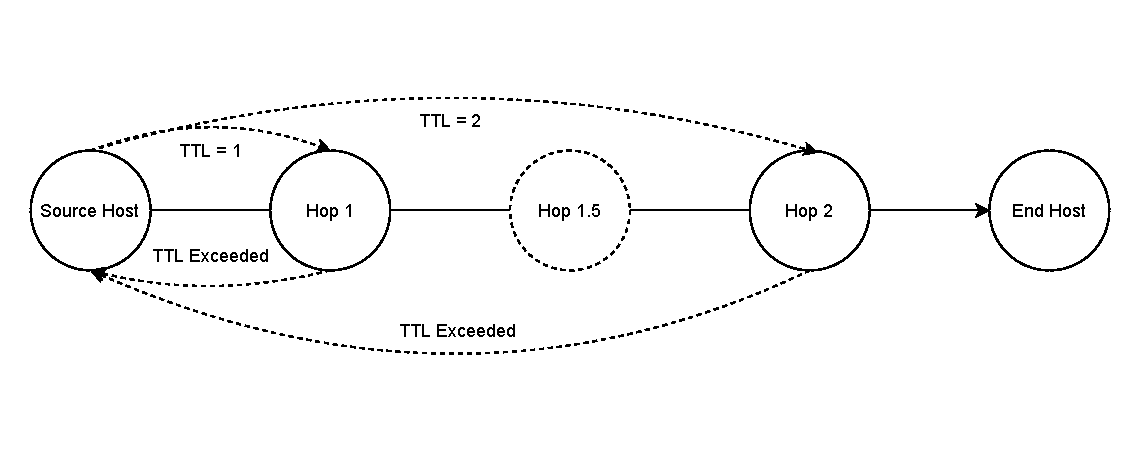
\includegraphics[width=14cm,keepaspectratio]{dissertation/images/ambig_icmp.pdf}
\caption{A diagrammatic representation of how ambiguities may arise with attributing ECT removal to a particular device on the network.}
\label{fig:icmp}
\end{figure}

Additionally, if we have a network interface, that is reasonably known to have cleared the ECN codepoint, we may also wish to ascribe the actions of this network interface to a particular Autonomous System (AS). This presents additional difficulties as router interfaces that comprise AS boundaries may utilise addresses from either of the adjacent AS's or some private address, the latter resulting in the resolution attempts failing.


\subsection{Generalizing to the wider network}
\label{sec:general}

As is generally seen as good scientific practice, we wish to obtain results that are on the whole generalizable. In the context of this paper, we seek to generalize the treatment of ECT codepoints within the wider network. For example, if we opted to obtain measurements from a singular host or vantage point on the network, we introduce a vulnerability to a particular device located close to the Host on the network that may erroneously clear ECT codepoints, potentially biasing the majority of the results obtained. Additionally, geographically close hosts, or hosts that share the same underlying Internet Service Provider (ISP). May share much of the same network level path to particular end hosts, hence are vulnerable to the same issues presented with collecting data from a singular vantage point on the network. 

Additionally, when we measure the network itself. We wish to measure a broad number of network paths, as a means to gather representative data of usage of the network, achieving this from a singular host on a given network is difficult, as it is likely the first few hops from a given host will be similar for the majority of connections given default routing behaviours.

With the following points being raised. We find it desirable to gather data from several vantage points on the network. Additionally these hosts would preferably distant to eachother with resepct the internet. Although not a directly comparable measure, geographically distant hosts usually satisfy this requirement.

\subsection{Identified Areas for Exploration}

In consulting the relevant literature for the topic of ECN modification on the network. We find that although a wealth of research exists in the area, the majority of research conducted, consults either ECT(0) for the majority of the measurements taken from the network in the case of <papers that use these>, or otherwise use the CE codepoint and do not subsequently elaborate on the specific remarking behaviour. As previously mentioned, RFC 1583 defines rightmost bit of the traffic class byte as to being set to zero, of which is now occupied by one of the two ECN bits. If this behaviour is still observed on the network, we would expect to see differential treatment of different codepoints on the network, hence this topic is to be pursued in the following chapters of this paper. Additionally, the recent development in regard to the implementation of ECN functionality within newer protocols such as Quic present potential deployment issues with devices that have not otherwise been exposed to ECT enabled UDP based traffic. We also present an additional area for elaboration. Does the transport protocol utilised influence the modification of ECT marked packets on the network? Hence we should seek to compare the incidence of whether TCP based or UDP based protocols are more prone to negative interactions with middle-boxes with resepct to ECN. Lastly, due to the nature of ECN measurement being inherently longitudinal in nature, we seek to provide an additional datapoint to the existing body of work that exists on the deployment of ECN. Hence we should also seek to discern the current adoption of ECN as well as instances of where ECN is otherwise inhibited on the network.


\section{Requirements}

With respect to the presented general problem, we highlight the existence of several requirements that were deduced during the course of the project and subsequently prioritised using the MoSCoW method to guide the development of project within the defined time constraints. Ensuring that the project met the initial criteria, answering the questions posed. MoSCoW prioritisation dictates that requirements be grouped into four distinct categories indicating their associated priority. They are as follows;

\begin{itemize}
    \item Must Have (\textbf{MH}), form the minimum usable subset of requirements, for the developed system to provide value
    \item Should have (\textbf{SH}), form important requirements but are not fundmanetal to the systems core function
    \item Could have (\textbf{CH}), form requirements that are desirable, but deemed less important than the above classifications
    \item Would be nice to have (\textbf{WH}), form requirements that were decided not to be delivered as a means to clarify scope of implementation.
\end{itemize}

\subsection{Functional Requirements}

\begin{itemize}
    \item \textbf{MH}: The tool should be able to generate traffic marked with any 4 variations of ECT codepoints in a given connection
    \item \textbf{MH}: The tool should generate data indicating whether ECT codepoints are removed during a TCP connections.
    \item \textbf{MH}: The tool should generate traffic mimicking a traceroute style connection under the Quic transport protocol
\end{itemize}



\subsection{Non-functional Requirements}

\begin{itemize}
    \item \textbf{MH} The developed tool should be readily deployable on both x86, and Arm based computers, as the tool is preferably deployed on a variety of arm based single board computers
\end{itemize}

\section{Summary}

In this chapter we have discussed the general problem domain around active network measurement with respect to ECN, we have discussed the rationale behind the general approach to measuring where on the network path ECN codepoints are stripped, and motivated the decision behind measuring individual ECT codepoints and transport protocols and their treatment on the network.




%==================================================================================================================================
\chapter{Design}
\label{chap:design}

Given the nature of the topic, we identify two high level aspects of design, that of the network analysis tool required to gather suitable measurements from the network, and the experimental design itself, to ensure that the measurements we gather from the network are both robust and are capable of answering the questions proposed in Chapter \ref{chap:analysis}.

\section{Network Analysis Tool}
\label{sec:tooldesign}

In order to gather the collection of measurements from the network, we require the design and subsequent implementation of a new network analysis tool. As described in section \ref{sec:requirements} the tool should support a multitude of protocols against the types of hosts identified in \ref{sec:method} of which is summarised in table \ref{table:proto}. Additionally we require that the tool be able to generate traffic using all of the available ECT codepoints. An overview of the operation of the tool in given in figure \ref{fig:tooldesign} where we highlight three high level components of design, isolating specific aspects of the requirements. We discuss several aspects of the tools proposed operation below, highlighting the distinct components that comprise the system.


\begin{figure}[H]
\centering
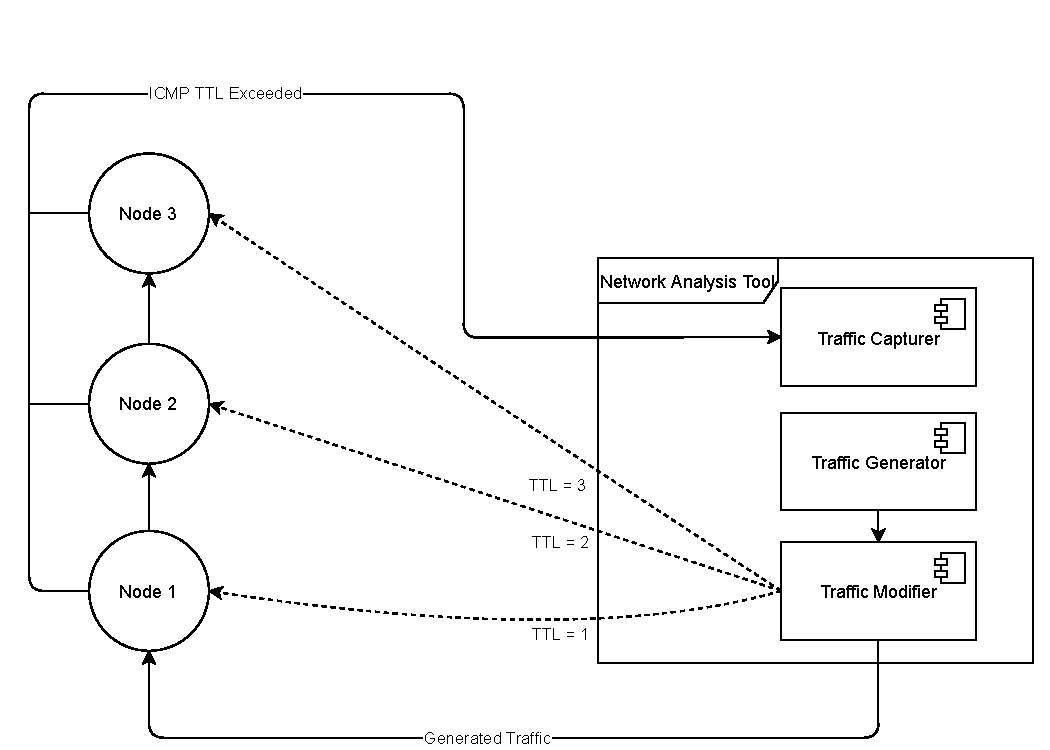
\includegraphics[width=14cm]{dissertation/images/sys_arch.pdf}
\caption{A diagrammatic representation of the proposed operation of the network analysis tool. Highlighting critical components for the tool's operation.}
\label{fig:tooldesign}
\end{figure}

\begin{table}[]
\centering
\begin{tabular}{|l|l|l|}
\hline
\textbf{Host Sample} & \textbf{TCP}          & \textbf{UDP}           \\ \hline
DNS Server  & DNS over TCP & DNS over UDP  \\ \hline
NTP Server  & HTTP/1.1     & NTP           \\ \hline
Web server  & HTTP/1.1     & HTTP/3 (Quic) \\ \hline
\end{tabular}
\caption{Summary of the connection types to conduct against each host sample to gather appropriate data}
\label{table:proto}
\end{table}

\subsection{Overview}

The proposed network analysis tool, should receive it's input from a text file. Ideally this text file should contain, Both an IP address, and an identifier describing what variant of host we are connecting against. Either DNS, NTP, or WEB. Given that the types of connection unto each of the hosts will be different. For each host to connect against, and each protocol used against that specific host, we seek to start connections using each ECT codepoint in turn. This can be achieved through the introduction of an 'application context' describing a state of the world for the system, informing the different components of the system how they are to operate. When starting a new connection. We push the application context unto each of the concerned components, describing the type of connection the system intends to carry out, informing the precise operation of the tool.

\subsection{Traffic Capture}

The traffic capturer component is responsible for recording the associated traffic unto a particular host. subsequently producing a file containing the packets observed during a connection, for subsequent analysis. The desired granularity of the captured traffic should be on the particular host, the type of connection being conducted, as well as the ECT codepoint being utilised on that given connection. This granularity can be achieved by successive notifications of the application context. The files produced should be semantically named to ensure ease in analysis of the generated files.

\subsection{Traffic Generator}

The traffic generator component is responsible for conducting the actual exchange of packets in order to attain the goals of the research. That is, this component is responsible for the implementation of several 'traceroute' style connections to hosts, such as sending a series of TTL limited packets unto a DNS resolver as described in section \ref{sec:icmp} that reflect a typical DNS request. This is convenient as if the packet is received by the host it is likely to respond to the request, allowing for the system to promptly halt and continue with the next connection.

\subsection{Traffic Modifier}

The traffic modifier component is responsible for receiving traffic generated from the traffic generator component and subsequently applying connection specific modifications to a given packet. This typically involves applying the correct ECT codepoint as required by the current state of the system with the exchange that the tool is attempting to conduct.

\section{Experimental Design}

\subsection{Host Selection}

To gain an understanding of the treatment of ECT codepoints on the wider network, we require a set of end-host samples to test against. These end hosts should be representative of usage of the internet, additionally it would be desirable if these hosts offered services over TCP as well as UDP, as we seek to uncover differences in treatment of ECT codepoints between transport protocols. We identify three distinct server populations to test against; DNS (Domain name service) resolvers, offering DNS services over both TCP as well as UDP. NTP (Network time protocol) servers, for which NTP operates over UDP, additionally the pool from which we select NTP servers from may optionally also deploy a web server operating over TCP. and Web servers, serving web content over TCP. Although web servers traditionally do not offer UDP based services, we see a growing adoption of Quic on the network, which we investigate in this paper.

We make a selection of all three server populations to test against. We randomly select a set of 1000 public DNS resolvers from \href{https://public-dns.info}{public-dns.info} on 08/01/2021. \href{https://public-dns.info}{public-dns.info} is a publicly available list of active DNS resolvers, that are periodically probed to ensure they are active. We select a subset of these DNS resolvers using the Unix \lstinline{shuf} command. In total we obtain 980 DNS resolvers that operate over IPv4 and 20 DNS resolvers that operate over IPv6.

Additionally we select the worlds top sites as indicated by the Alexa top sites list as of 08/01/2021. We remove domains from the provided list that are associated with categories of material such as pornography or gambling using the University of Toulouse's open domain blacklist. This was conducted as a means to avoid implications with certain deployment locations such areas of the Middle East as well as avoiding interference from various ISPs with IP based content filters. The filtered list of domain names were subsequently resolved on the same day using google's public DNS resolver 8.8.8.8 with the \lstinline{dig} command to both IPv4 as well as IPv6 addresses if available until 1000 total IP addresses were obtained. This resulted in the generation of a dataset of 864 IPv4 addresses and 126 IPv6 addresses.

To obtain a set of public NTP servers we utilise the \href{https://www.pool.ntp.org}{NTP pool}, a virtual cluster of NTP servers providing precision timekeeping. Attempting to resolve \lstinline{pool.ntp.org} through a DNS resolver returns the IP address of a given NTP server from the pool. The returned IP address changes every few minutes through the implementation of a round robin DNS. The pool supports the discovery of geographically bound hosts through attempting to resolve pool.ntp.org with an applicable region as a subdomain, for example. Attempting to resolve europe.pool.ntp.org will attempt to return an NTP server located in europe. We utilise this approach to obtain hosts that are geographically distributed. Additionally the ntp pool offers additional subdomains that offer IPv6 addresses of NTP servers to be obtained. It was discovered that 2.ntp.pool.org is one of these domains.
Hence we implement a simple shell script to collect IP addresses from the resolution of \lstinline{pool.ntp.org} under all region codes across a period of 2 months beginning from 20/10/2020. We subsequently randomly select 1000 of the returned address using the \lstinline{shuf} command. In total 679 IPv4 addresses and 321 IPv6 addresses were collected.

Lastly, in figure \ref{fig:locs} we present the approximate geographic distributions of the gathered hosts as indicated by Maxmind IP Geolocation. However these resolutions are subject to limitations of mapping IP addresses to specific locations as suggested by <paper>. We find that there is reasonable geographic coverage offered by the hosts, as discussed in chapter \ref{chap:analysis} which helps assure that a reasonable variety of pathways on the network are tested. However, the selection of web server hosts offered, appears clustered to a few isolated areas in the United States, Europe and East Asia.

\begin{figure}[H]
    \centering
    
    \begin{subfigure}[b]{\textwidth}
         \centering
         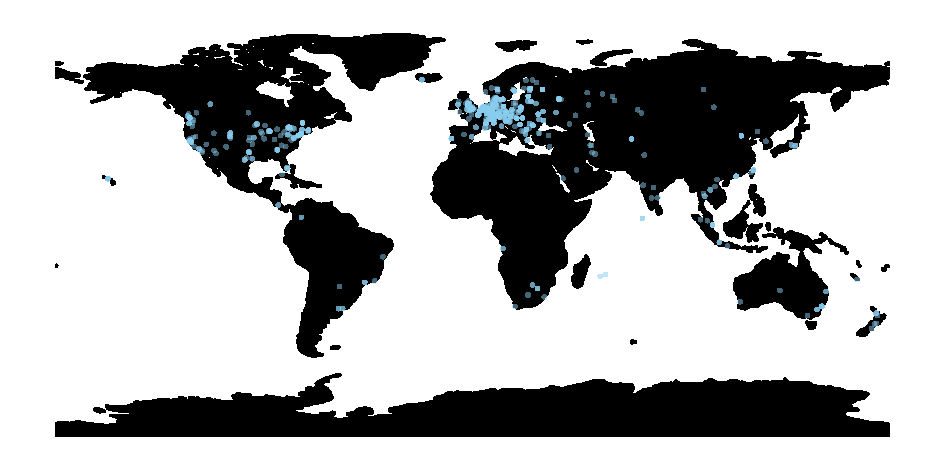
\includegraphics[width=0.5\textwidth]{dissertation/images/ntp.locs.map.pdf}
         \caption{}
     \end{subfigure}
     
     \centering
\begin{subfigure}{.5\textwidth}
  \centering
  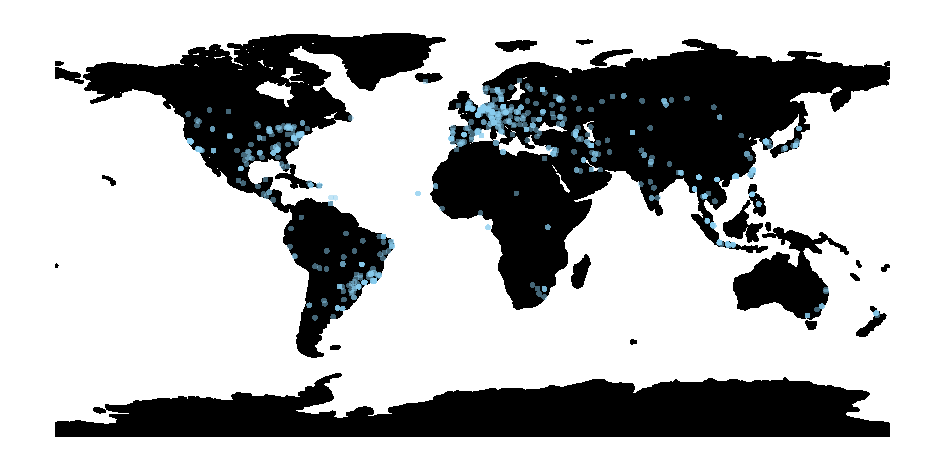
\includegraphics[width=\linewidth]{dissertation/images/dns.locs.map.pdf}
  \caption{}
  \label{fig:sub1}
\end{subfigure}%
\begin{subfigure}{.5\textwidth}
  \centering
  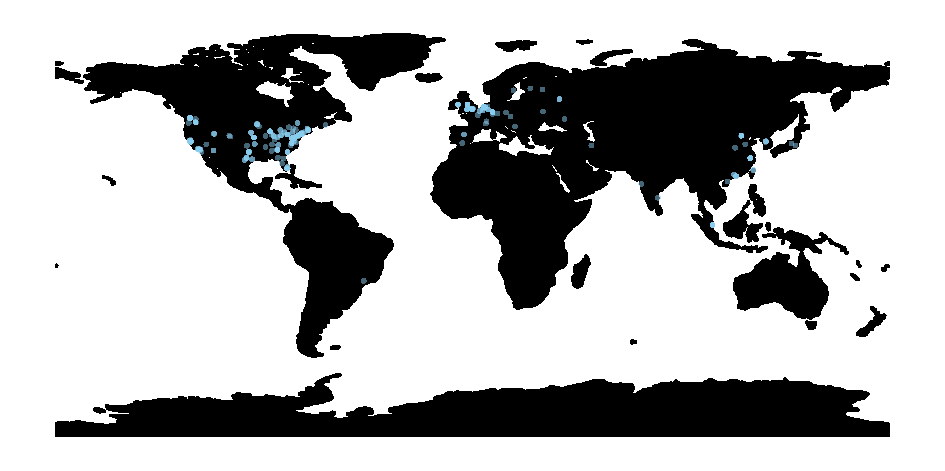
\includegraphics[width=\linewidth]{dissertation/images/web.locs.map.pdf}
  \caption{}
  \label{fig:sub2}
\end{subfigure}
\caption{Approximate locations of each server population, as indicated by MaxMind IP Geolocation as of 29/01/2021, (a) NTP Servers, (b) DNS resolvers, (c) Web servers}
\label{fig:locs}
  
\end{figure}

With respect to the discussion in section \ref{sec:general}, we recognise that it is desirable to gather data from multiple vantage points on the network. We select from two main bodies of possible vantage points from which to conduct measurements from. Firstly, we select a collection of hosts operated by AWS (Amazon Web Services). This is allows for us to utilise a variety of hosts located geographically distant from another. We also recruit student participants as part of an ethics approved study, as means to gather data from residential networks. Additionally as another vantage point, the author opted to deploy the tool within their own residential network to gather additional measurements.

\subsection{Measurements}

Having selected a collection of sample hosts to test against, and a selection of hosts to run the network analysis tool from. We must also concretely define the type of connections that we seek to conduct to answer the questions posed in section \ref{sec:questions}. The underlying protocols to be used for a given type of server can be seen from \ref{table:proto}. For each server we intend to test against, we should. For each protocol, both UDP and TCP, we must conduct traceroute style connections unto the host as decribed in section \ref{sec:icmp}. with all 4 variants of ECT codepoints that are available. We may use the variant of a 00 codepoint as a means to determine whether the host is operational, and is listening on a given port. Additionally to provide resistance against transient network outages and other undesirable scenarios encountered during deployment, we may wish to run the collection of data from all of the hosts identified multiple times. It was empirically measured that the dataset of source hosts to test against requires slightly under 2 days to complete. Hence, it was determined a total runtime of 2 weeks should be sufficient to attain suitable measurements from the network. Using the this approach we should attain appropriate data to answer the questions proposed in section \ref{sec:question}.


{{Overview of specifics of traffic generated}}
{{What types of connection for each host}}
{{ECT markings on each connection}}


% what we need to measure -> design of experiemnt
% how we measure it -> design of tool
% where deploy in many places -> choice of aws and participant locations

% {{Create a graph with graphviz to visualise how tool components interact with eachother and the wider network ie. system architecture diagram}}

% {{Small discussion of the high level components of the tool}}
% {{Traffic generator}}
% {{Traffic modification}}
% {{Traffic capture}}


%==================================================================================================================================
\chapter{Implementation}

This chapter discusses the implementation of the network analysis tool, discussing the underlying approaches used to gather the appropriate data from the network. We also discuss the tool's subsequent deployment as means to gather the measurements from the network to inform the Chapter \ref{chap:evaluation}.

\section{Network Analysis Tool}

The tool was naturally realised as a concurrent system. Each of the previously identified components identified in Chapter \ref{chap:design} were modelled as their own thread of execution with minimal interactions between them. The system was implemented in the C programming language given its relatively small footprint ensuring ease on deploying on resource limited Arm based computers, and the availability of underlying libraries to implement essential functionality required by the system.

\subsection{Traffic Capture}

The traffic capture component was realised as a relatively simple application of libpcap. An open source library supported under most Unix(-like) operating systems, that allows for the live capture of network traffic. Additionally, this library supports traffic filtering rules, ensuring that the only traffic observed by the component during a connection relates to the connection that the system is currently conducting, this was employed to simplify subsequent analysis of the data produced. The component exports a relatively basic API, in order to support the operation realised in chapter \ref{chap:design} and is summarised in listing \ref{lst:pcapapi}. The component opens a semantically named file describing the connection upon receiving an application context through the \lstinline{pcap_push_context} function, and will commit packets to this file until the component is notified that the connection in question has ended through \lstinline{pcap_close_context}, subsequently closing the file.

\begin{lstlisting}[caption={The exported API of the traffic capture component to facilitate the live capture of traffic generated by the system.}]
struct pcap_controller_t * pcap_init();
void pcap_push_context(
    struct pcap_controller_t *pc,
    struct connection_context_t *ctx
);
void pcap_wait_until_rdy(struct pcap_controller_t *pc);
void pcap_close_context(struct pcap_controller_t *pc);
void pcap_free(struct pcap_controller_t *pc);

\end{lstlisting}

\subsection{Traffic Generator}
\label{sec:impltg}

The traffic generator component utilises a variety of approaches to attain the goals of the research, we largely rely on the POSIX networking api to implement much of the functionality required by the research. We implement a variety of functions intended to receive a buffer and subsequently populate this buffer with a valid request targeting one of the specific host populations, such as DNS resolvers. The buffer is then passed to a generic traceroute method, which implements the process described in section \ref{sec:icmp}. Starting from a TTL of 1 through to 64, we send a maximum of three packets onto the network, after each packet is sent. We check whether an ICMP TTL exceeded response message has been returned, furthermore we match the ICMP response against the current connection, comparing the port number received from the ICMP quotation and the port number used to send the request. If such an ICMP response is received or if the maximum number of retries is reached, we increment the TTL. If we receive a response from the end host we are sending the traceroute to, we simply abort the rest of the traceroute operation and continue with the next connection.

\subsection{Traffic Modifier}

The traffic modifier component heavily utilises the libnetfilter\_queue library. A Linux library allowing for arbitrary userspace modifications of packets that have been queued by the underlying operating system kernel. This is convenient, as this allows us to both, circumvent limitations in place as a result of the operating system kernel and the POSIX networking API or otherwise avoid the pervasive use of raw sockets in most scenarios. For instance, the mechanism to enable ECN under TCP on Linux requires the use of the \lstinline{sysctl} utility or equivalent, and only allows the ECT(0) codepoint to be utilised during connections, which is undesirable with respect to the research aims. Alternatively we may opt to implement a minimal TCP networking API in userspace which was also deemed undesirable. libnetfilter\_queue simplifies this process by allowing us to leverage the functionality we require from other utilities such as the kernel's networking stack and extend it as packets are about to be sent on the network. For instance, listing \ref{lst:libnf} shows how arbitrary ECT codepoints may be used under a TCP connections using libnetfilter\_queue. where the \lstinline{ctx} variable defines the applications current context to inform its operation.

Other approaches, such as those used by \cite{bauer_measuring_2011} used iptables to apply modificataions to the traffic class byte to packets that satisfied a given set of rules. However as we require granular control over the ECT codepoint at runtime, as the codepoint will vary from connection to connection. This was deemed insufficient.

\begin{lstlisting}[caption={A demonstration of userspace modification of the traffic class byte on packets queued by the operating system kernel for transmission on the network.}]
struct iphdr *ip4 = nfq_ip_get_hdr(pkt);

        if (ip4)
        {
                ip4->tos = 0;

                if (IS_ECN(ctx->flags) && 
                    ((!hdr->syn && !hdr->fin && !hdr->rst))
                        ip4->tos = ctx->flags;

                nfq_ip_set_checksum(ip4);
                nfq_tcp_compute_checksum_ipv4(hdr, ip4);
                return_value = 0;
        }
\end{lstlisting}
\label{lst:libnf}


\subsection{ECT modifications with TCP}

A noted aspect of functionality under the system should be the generation of traffic that would denote whether ECT codepoints are removed during a TCP connection. To attain this we utilise a mixture of functionality provided by each of the components that comprise the system. We begin by starting a standard TCP connection unto a given host. We rely on the traffic modifier component to observe the outgoing SYN segment of TCP connection establishment, and subsequently storing the sequence number associated with the segment. If the host responds, the traffic capturer component will subsequently receive a segment containing the TCP SYN ACK segment of TCP connection establishment. We subsequently store the associated acknowledgement number associated with the connection. The traffic generator component uses these provided values, and opens a raw network socket. Formatting a standard TCP data segement utilising the provided sequence and acknowledgement numbers, and begins a traceroute as described in section \ref{sec:impltg}. This processis breifly summarised in listing <n>. The rationale behind this approach allows us to suitably imitate a standard TCP connection as far as the scope of network is concerned. Additionally this allows us to avoid writing the majority of TCP networking stack, circumventing a variety of limitations such as lack of access to a TCP connections associated sequence and acknowledgement numbers, as well as hard coded in kernel re-transmission behaviours, which prevents us from utilising any simpler approaches.

\begin{lstlisting}[caption={A demonstration of launching traceroutes during a TCP connection, implementation details such as the use of synchronisation primitives and error checking have been omitted for the sake of brevity}]

uint8_t buff[TCP_SZ];
uint8_t data[DATA_SZ];

connect(fd, &hostaddr, hostaddrlen);

int seq = nf_get_seq_number();
int ack = pcap_get_ack_number();

format_tcp_header(seq, ack, &buff, &data);
do_traceroute(&hostaddr, &buff);

\end{lstlisting}


\subsection{Traceroutes under Quic}

The chosen implementation of Quic used for the tool was lsquic by litespeedtechnologies, this was deemed appropriate as it features a library for the C language, as well as featuring native support for ECN. Such as implementing support for ECN ack frames as described in chapter \ref{chap:background}. As version negotiation under Quic is yet to be standardised, we empirically measured the best supported Quic version at the time that implements ECN functionality. It was measured that ietf-draft-29 was the best supported and was subsequently selected for the implementation of the network analysis tool. Due to time constraints, modifying lsquic to support a native implementation of traceroute was deemed out of scope. Hence, we proceed as follows in the implementation of a traceroute mimicking a Quic connection. 

We begin by creating a standrd UDP datagram network socket, and subsequently set the TTL of the socket to 1 using the \lstinline{setsockopt} function. We then start the lsquic library, passing in the previously constructed datagram socket, with a TTL of one. We attempt to establish a connection unto the desired host using this socket under lsquic. This subsequently results in lsquic generating connection establishment packets intended for the host. The traffic modifier component, which would normally apply connection specific modifications observes these generated packets the operating system is intending to send. Under this component we access the contents of the UDP datagram, copying teh contents to a buffer which is shared between the traffic modifier and generation components. When the connection subsequently fails, as the TTL of the socket utilised is 1. We now have a cached Quic packet observing the correct semantics for that host. We then utilise the same file descriptor and the acquired buffer containing a Quic connection establishment packet in a standard traceroute operation. listing <n> summarises this approach as implemented in the network analysis tool.

\begin{lstlisting}[caption={A demonstration of launching traceroutes under Quic, leveraging support from lsquic to generate a suitable connection establishment packet, which is then utilised under a standard traceroute operation. The use of synchronisation primitives and error checking have been removed for the sake of brevity.}]

int send_quic_http_probe(
    int fd, 
    char *host, 
    char *sni, 
    int locport, 
    int ecn, 
    struct quic_pkt_t *relay)
{
  
  struct sockaddr_storage addr;
  socklen_t socklen;
  uint8_t *pkt_relay = relay->pkt_relay;
  host_to_sockaddr(host, PORT_TLS, &addr, &socklen);
  
  // send and capture connection establishment
  send_generic_quic_request(fd, host, sni, locport, ecn, 1, NULL);
  ssize_t pkt_relay_len = relay->pkt_relay_len;
  
  // Do traceroute operation
  ... 
}

\end{lstlisting}

\section{Deployment}


\subsection{Overview}

Following the development of the network analysis tool, we seeked to attain a set of measurements from the network as described in chapter \ref{chap:design}. To do this we conducted a medium scale deployment of the developed tool for a period of two weeks utilising a variety of hosts from both datacentres and residential networks from a variety of geographic locations. The deployment was launched on the 11/01/2021, and subsequently ended two weeks later on the 29/01/2021.


\subsection{Datacentre hosts}

To facilitate the deployment of the tool across a large number of AWS hosts we utilise the suite of software provided by Hashicorp. Two specific tools that we utilise are Packer and Terraform. We discuss each tool in turn.

Packer was utilised as a means of automating the creation of virtual machine images containing the network analysis tool, automatically distributing them to a storage medium accessible via AWS for subsequent deployment. The virtual machine images utilised Ubuntu 20.4 as their substrate with the network analysis tool subsequently being installed within the virtual machine image through a shell script, performing the tools required setup. Additionally to correctly schedule the running of the tool. A cron job is scheduled within the virtual machine image to start the first iteration of the tool at midnight and fix the running of the tool every second calendar day that the virtual machine instance is up. This roughly corresponds to the 2 day run time per iteration of the dataset which was empirically measured prior to deployment.

Once a suitable virtual machine image was produced, Terraform, an infrastructure as code tool allowing for multi-region deployments on the AWS platform was utilised to bring up several AWS instances at once. The precise regions used is summarised in table <n>. We provision each virtual machine in use with a basic set of additional infrastructure. We provide each virtual machine image with both a public IPv4 and IPv6 address. In regards to firewalling, we allow traffic from any source on any port towards the virtual machine, although heavy handed, this prevents any potential issues with returned ICMP responses being filtered by default configurations of AWS infrastructure. This deployment to many geographic locations was implemented through the use of a parameterised terraform module.

As no thorough integrations between packer and Terraform exist outside of using environment variables, a Python script was produced, that would parse the output from Packer, identifying applicable virtual machine image IDs, subsequently producing a json file containing terraform variables. Listing <n> demonstrates this approach of integrating the output of packer with terraform to succinctly utilise produced virtual machine images within a parameterised terraform module.

\begin{lstlisting}[caption={A demonstration of extracting produced virtual machine image IDs from packer, subsequently producing a data file amenable for use within Terraform.}]

out_stream = subprocess.check_output([
                            "packer",
                            "build",
                            "-machine-readable",
                            file
                            ])
lines = out_stream.decode("utf-8").split('\n')
out_json = None

for line in lines:
    tokens = line.split(',')
    timestamp,target,category,*data = tokens
    
    # Find line containing virtual machine IDs
    if target != "amazon-ebs" or category != "artifact":
        continue
    
    ret = get_ami_from_data(data)
    if not ret:
        continue

    out_json = ret
    break

with open("images.auto.tfvars.json", 'w') as f:
    json.dump(out_json, f)

\end{lstlisting}


\begin{table}[H]
\centering
\begin{tabular}{|l|l|}
\hline
\textbf{\begin{tabular}[c]{@{}l@{}}AWS Region\\ (Location)\end{tabular}} & \textbf{EC2 Instance type} \\ \hline
\begin{tabular}[c]{@{}l@{}}eu-west-2\\ (London)\end{tabular}             & t2.medium                  \\ \hline
\begin{tabular}[c]{@{}l@{}}me-south-1\\ (Bahrain)\end{tabular}           & t3.medium                  \\ \hline
\begin{tabular}[c]{@{}l@{}}sa-east-1\\ (São Paulo)\end{tabular}          & t3.medium                  \\ \hline
\begin{tabular}[c]{@{}l@{}}af-south-1\\ (Cape Town)\end{tabular}         & t3.medium                  \\ \hline
\begin{tabular}[c]{@{}l@{}}us-east-1\\ (North Virginia)\end{tabular}     & t2.medium                  \\ \hline
\begin{tabular}[c]{@{}l@{}}us-west-1\\ (North California)\end{tabular}   & t2.medium                  \\ \hline
\begin{tabular}[c]{@{}l@{}}ap-northeast-1\\ (Tokyo)\end{tabular}         & t2.medium                  \\ \hline
\end{tabular}
\caption{Summary of AWS locations used as vantage points in the deployment of the network analysis tool. Paired with the instance type used within that AWS region.}
\end{table}


As previously mentioned, student participants volunteered to deploy the tool within their own networks as part of an ethics approved study. In total 4 participants were recruited in assisting with the goals of the research. All of the participants opted to use a variant of the Raspberry Pi to deploy the tool within their own networks. Particpants were assisted in installing the tool, and provided with a shell script which would compile and install the tool on their behalf. Similarily to the AWS hosts. This installation script would orchestrate itself through the use of cron to begin running at midnight from the moment that the tool was installed. Subsequently running every two calendar days for the duration of the research period. In table \ref{table:participants} we present an alias for each participant and the approximate geographic location for each participant in the study, we use these aliases consistently throughout the rest of the paper.


\begin{table}[H]
\centering
\begin{tabular}{|l|l|}
\hline
\textbf{Participant Alias} & \textbf{Geographic Location}    \\ \hline
Participant-1     & Glasgow, Scotland      \\ \hline
Participant-2     & , Japan                \\ \hline
Participant-3     & , Estonia              \\ \hline
Participant-4     & , United Arab Emirates \\ \hline
\end{tabular}
\label{table:participants}
\caption{Approximate geographic locations for each participant that took part in the study. We find a respectable geographic coverage, although lacking residential vantage points located in the Americas.}
\end{table}

%==================================================================================================================================
\chapter{Results} 

In this section we discuss the results from the measurements obtained in chapter \ref{chap:implementation}. Evaluating the current status of adoption of ECN on the network, and identifying where on the network devices remove ECT codepoints.

\section{ECN under TCP}

\subsection{ECN adoption}

In addition to discovering where ECN markings are removed on the network, we seeked to uncover the current status of ECN adoption on the network. Across all vantage points, we select the probes unto hosts that launched TCP connections in an attempt to trace the traversal of ECT(0) codepoints across the network. In these operations, during connection establishment we attempt to negotatiate ECN as described in section \ref{sec:ecntcp}. We analyse the files inspecting where the returned SYN-ACK as part of connection establishment also sets the ECE bit of the TCP header indicating that the end host intends to use ECN. As we have several traces of the dataset perhost, we average across each trace within hosts, before subsequently averaging across all hosts. We present our findings in table \ref{table:ecnnego}.

\begin{table}[H]
\centering

\resizebox{0.4\textwidth}{!}{\begin{tabular}{|l|l|l|}
\hline
\multirow{2}{*}{Host Sample} & \multicolumn{2}{l|}{ECN Negotiated} \\ \cline{2-3} 
                             & IPv4             & IPv6             \\ \hline
DNS Resolvers                & 82\%             & 90\%             \\ \hline
NTP Servers                  & 80\%             & 88\%               \\ \hline
Web Servers                  & 79\%             & 86\%                 \\ \hline
\end{tabular}}
\caption{Percentage of hosts willing to negotiate ECN by Host sample and IP version utilised. We notice no appreciable difference in ECN adoption between host samples, and a slight increase between IPv4 hosts to IPv6 hosts of the same host sample.}
\label{table:ecnnego}
\end{table}

As other research has indicated we see a general increase over time in the willingness for hosts to negotiate ECN over previous time periods. Furthermore we notice an increase in willingness to negotiate ECN between hosts that operate over IPv6 when compared to IPv4.  We present our findings against other measurements that have been conducted over previous years. We see that our results are largely inline with the growth of the willingness to negotiate ECN in hosts. Of which is summarised in figure \ref{fig:ecngrowth}. We do however notice an apparent plateau in the growth of willingness to support ECN in hosts when we compare our additional datapoint to the next most recent measurement (\cite{mcquistin_is_2015}) which recorded willingness to negotiate ECN amongst measured hosts at 82\%, whilst our measurements average at a similar percentage of <percentage>. This may suggest an apparent levelling of the deployment of ECN, albeit the results we obtain for IPv4 based hosts are still considerably lower than that of IPv6 based hosts.

\begin{figure}[H]
    \centering
    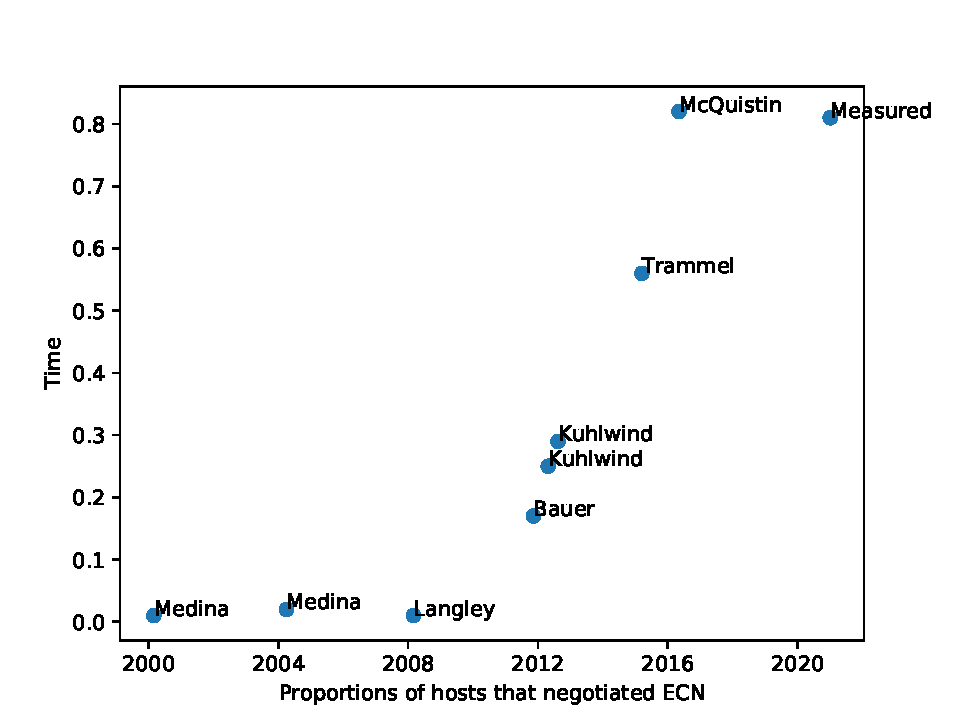
\includegraphics[scale=0.7]{dissertation/images/ecn_trends.pdf}
    \caption{Graph showing relative proportions of IPv4 hosts that would negotiate ECN over time. Noting an apparent plateau in the growth of hosts willing to negotiate ECN.}
    \label{fig:ecngrowth}
\end{figure}

% Discuss more in specifics of the papers that we include in the graph %





\subsection{Are ECT codepoints removed during TCP Connections}

Using a new approach through the implementation of a new network analysis tool, we seeked to measure whether ECT codepoints were removed during a TCP connection. For each host sample we select traces unto a given host under ECT(0). We iterate over the ICMP responses present in the trace inspecting the associated quotation's included IP header checking whether the ECT codepoint has a value of zero. We present our findings in figure \ref{fig:ect_strip}.

\begin{figure}[H]
    \centering
    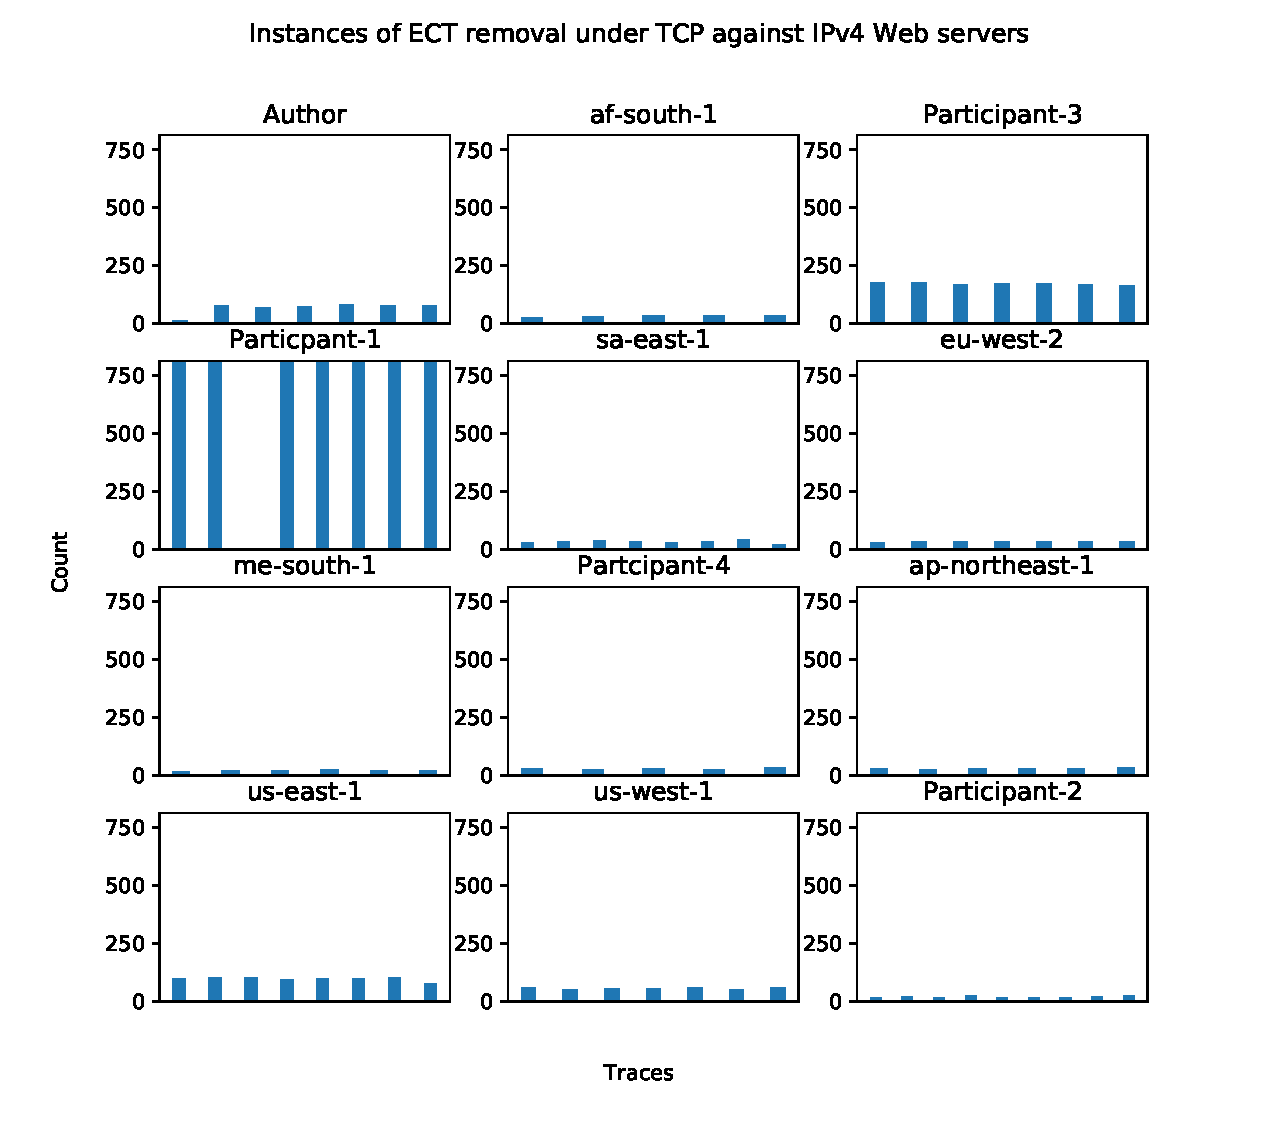
\includegraphics[scale=0.7]{dissertation/images/tcp_bar.pdf}
    \caption{Bar graphs presenting how instances of devices on the network clearing the ECT(0) field. We present data on the granularity of a singular host. We see the presence of a singular outlier that experiences ECT removal on all outbound connections.}
    \label{fig:ect_strip}
\end{figure}

What is immediately clear from our findings, is that an individual participant experiences ECT removal on all outbound connections utilising TCP under at least port 80. Effectively prohibiting all ECN enabled traffic from functioning at all from this vantage point in the network. This was to be expected as localised individual devices have been identified in the past <cite paper planet lab node>. Outwith this individual host we find the occurrence of removal of ECT(0) during connections to be relatively rare, we identify this finding as an outlier and subsequently remove this vantage point from further data aggregations as a means to prevent biasing results. We identify that although varying between vantage points, with some experiencing ECT removal more often than others. On average, approxiamtely ~0.5\% of connections experience removal of the ECT(0) codepoint during connections. This is relatively consistent with the results found from <paper> who found that around <n> TCP connections towards web server hosts also experience this behaviour.






\subsection{Where are ECT codepoints removed on TCP connections}

In addition to detecting when ECT codepoints were removed during TCP connections, we additionally seeked to ascertain where ECT codepoints were being removed on the network. The results from sample trace data unto a particular host has been presented visually in figure \ref{fig:traces}.

\begin{figure}[H]
    \centering
    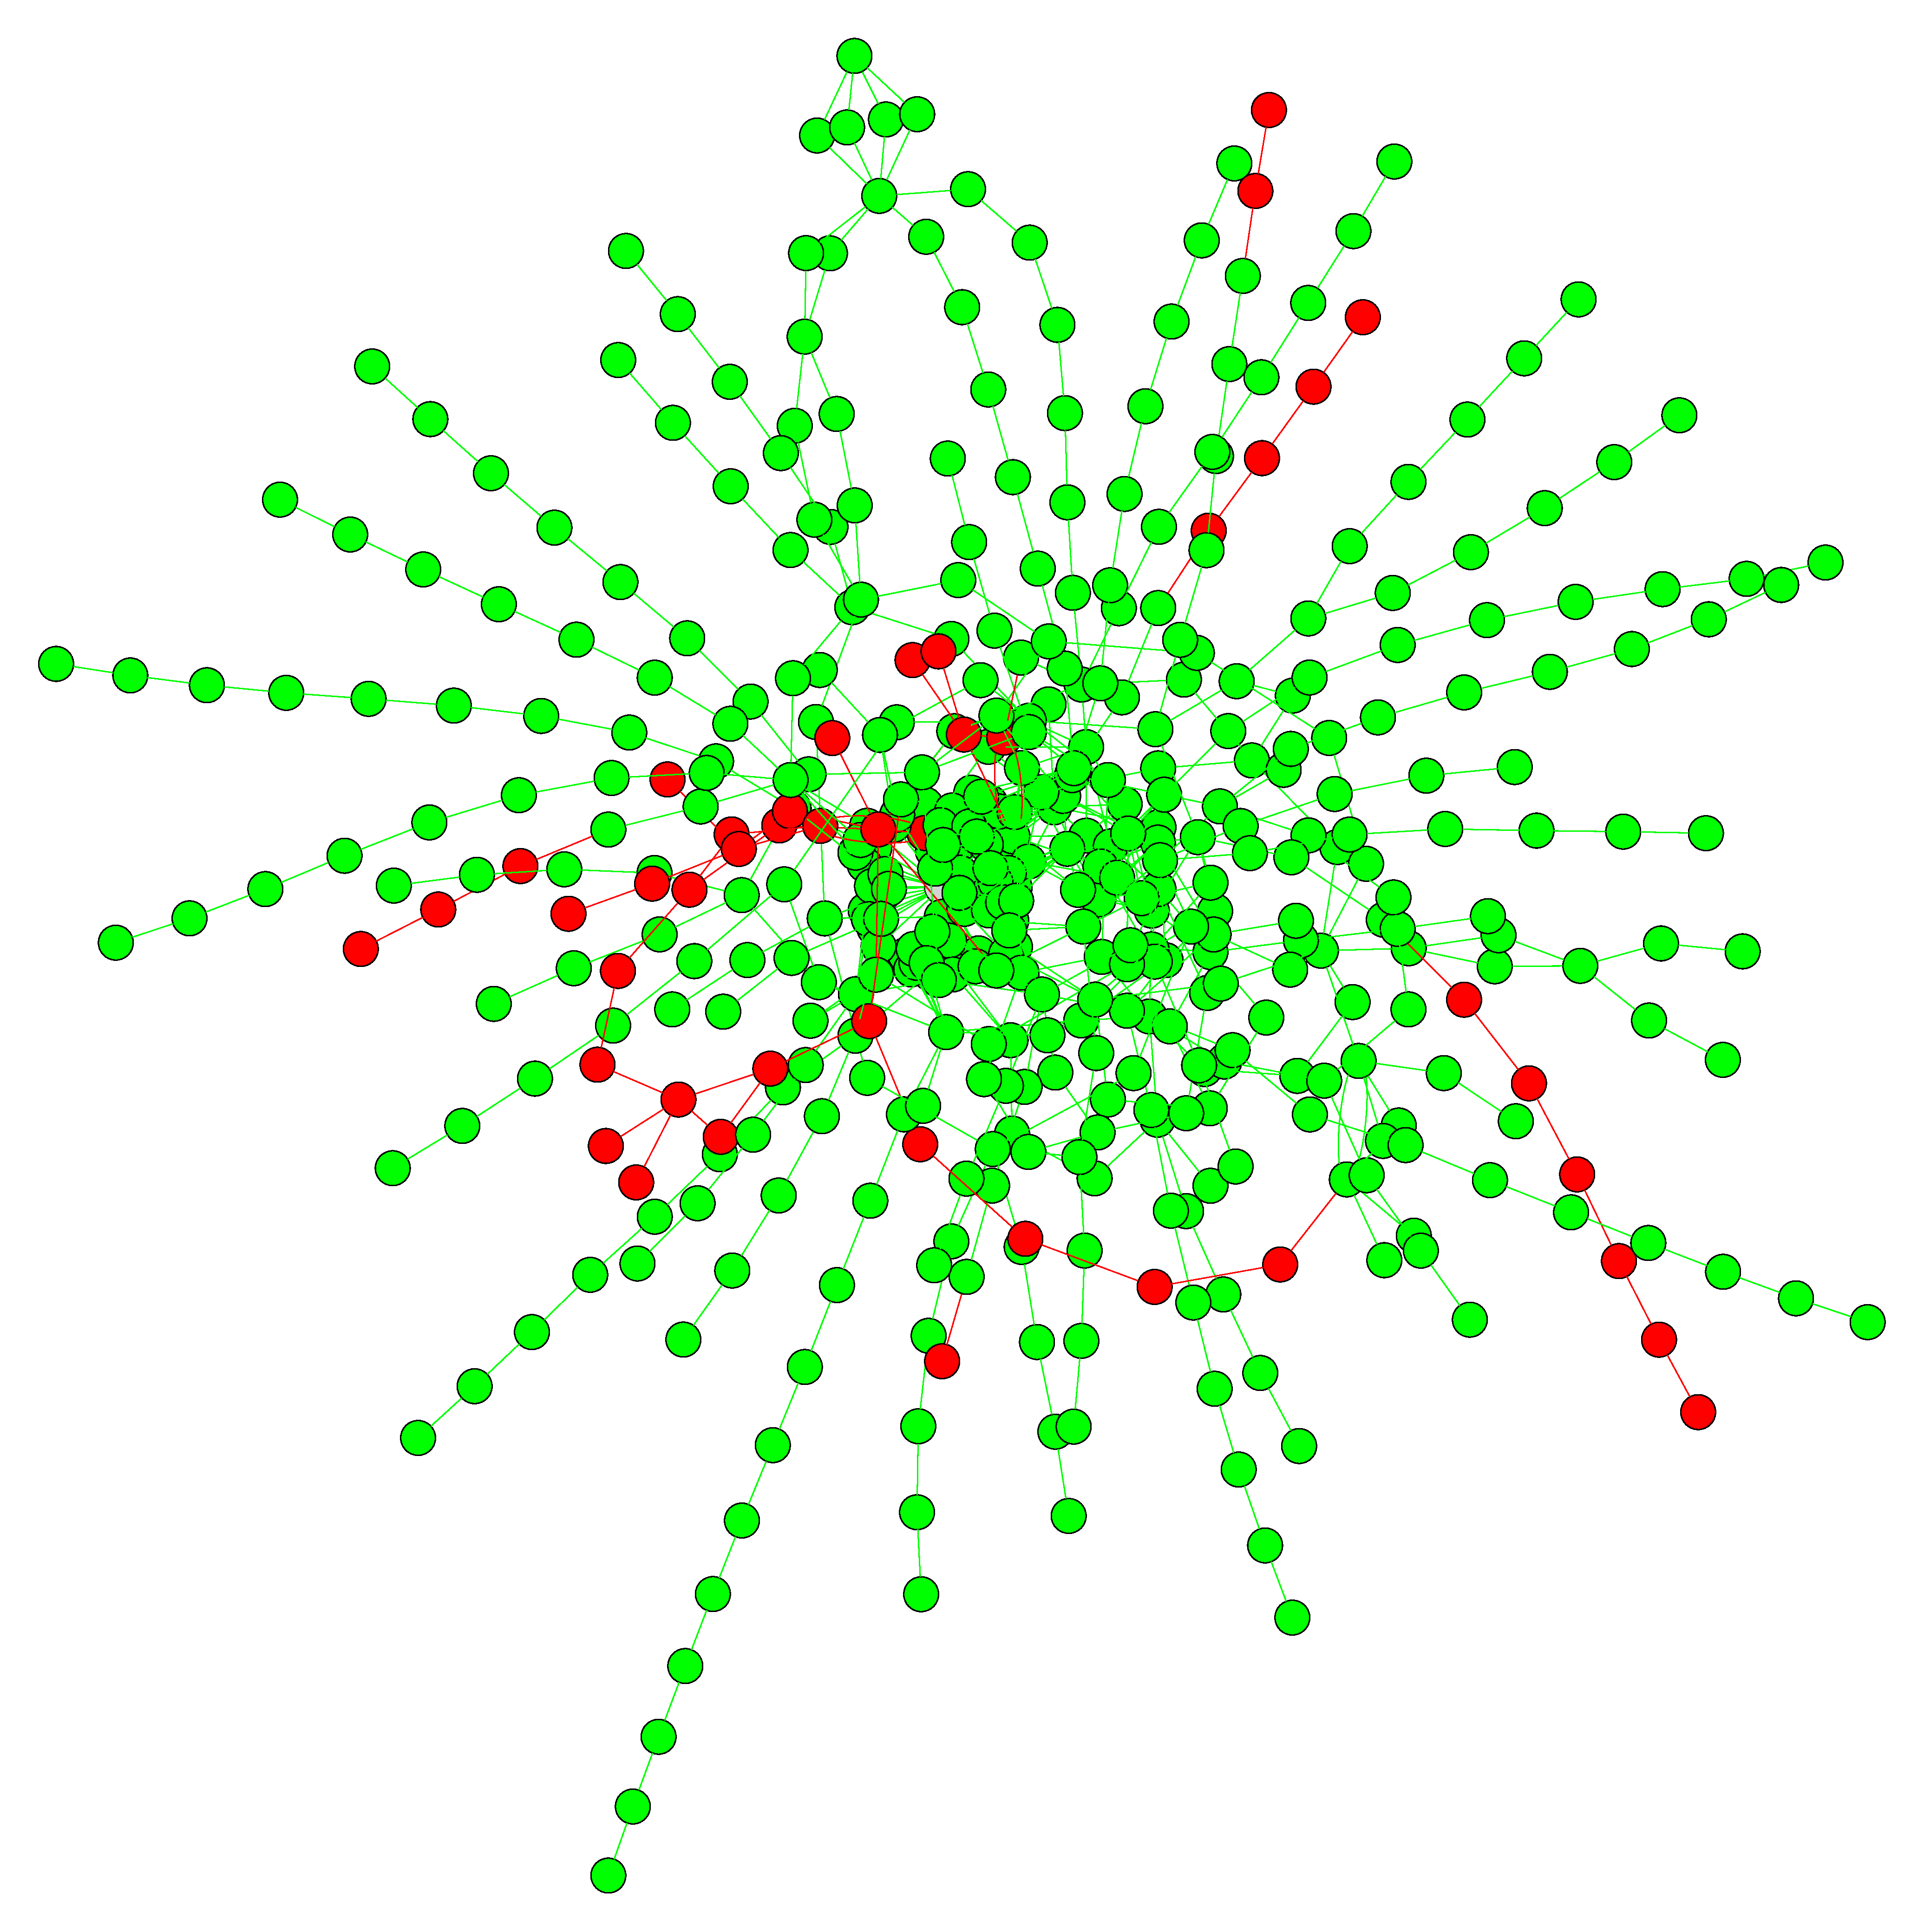
\includegraphics[scale=0.1]{dissertation/images/hops.pdf}
    \caption{Visualization of network level hops showing interface hops where the ECT codepoint is not preserved being shown in red, vantage points on the network are shown in grey, and the intended host being shown in blue. In most instances the responsible device appears far from the vantage point, under this particular host.}
    \label{fig:traces}
\end{figure}


\section{ECN under UDP}

In addition to observing modifications of ECT fields under TCP, we seeked to investigate modifications under UDP, this was to determine whether there were potential deployment issues with Quic. A new transport protocol that has introduced support for ECN. As well as to determine whether transport protocols are equivalent under ECN remarking behaviours. We present our findings in the following sections.

\section{A cursory look at Quic}

As noted in section \ref{sec:aims} we seeked to investigate the state of the operation of ECN under Quic. Hence, a traceroute operation was implemented that mimicked connection establishment under Quic. We present findings relating to the current status of the deployment of Quic, additionally presenting the current status of the deployment of ECN within Quic. Similarly to TCP we additionally discover if and where devices on the network clear the ECN field as Quic connection establishment packets traverse the network.

In gauging the adoption of Quic under the web server hosts that we selected as part of the dataset. We select Quic traces that utilise the codepoint "00" unto each web server host. We define a host as supporting ECN as one that at least responds with a UDP Quic packet in response. We find that across 1000 web server hosts, a total of <n> hosts supported ECN, with a total of <n> IPv4 hosts and <n> IPv6 hosts respectively. Overall, we have a proportion of 0.034\% of hosts having adopted Quic. This suggests relatively minimal deployment of Quic. However as Quic is a relatively new protocol, we would expect the proportion to be relatively low.

In determining the deployment of ECN under Quic, we select traces utilising, the ECT(0) codepoint under each webserver host. We define a host as supporting both Quic and ECN if the the host both responds, and in one of the response packets sends at least some variant of the ECN ack frame, as defined by Quic, or otherwise mark returned packets with a non zero ECT codepoint. In total we find that none of the hosts measured supported ECN under Quic, again. This is likely to be expected due to the relative immaturity of the deployment of Quic.


\section{Are Transport Protocols equivalent under ECN?}

\section{Are IP versions equivalent under ECN remarking?}


\section{Other notable behaviours}

Across the traces gathered from each host, it was noticed that in certain cases ICMP responses from the network as part of a traceroute operation were received that were marked with a given ECT codepoint. This is interesting as ICMP does not utilise ECN and it would be expected that devices sending ICMP responses would not subsequently utilise the field.

We investigate the specific behaviour of devices on the network in regarding to devices apparently sending ECT marked ICMP responses. We note that the majority of connections exhibit this behaviour from at least a singular device. Additionally the actual number of devices that observe this behaviour is likely slightly higher. As the reverse path from a host towards a given vantage point may also clear the ECT fields.

We consult the available literature to determine a root cause for this behaviour, and to the best of the authors knowledge this behaviour may originate from misconfigured devices derving behaviour from RFC ..., which suggests that devices sending ICMP response messages should set the Type of service field to the same value as the packet that resulted in the ICMP response being generated. Notably ICMP TTL exceeded are not considered ICMP response messages. Hence it is not clear why devices are behaving in this manner.

However, this behaviour has many interesting implications. This behaviour may be used to identify devices on the network that continue to use TOS semantics, as this marking behaviour is derived under this field. Additionally, our measurements are limited to path transparency on the forward path. If devices can be identified that mark packets with the ECT codepoint in generating ICMP TTL Exceeded responses. This may allow for some path transparency measurements to be additionally determined on the reverse path (from a host towards a given vantage point), notably without any cooperation from the host being measured. A common limitation in the available literature of network measurement.

\section{Discussion}

%==================================================================================================================================
\chapter{Conclusion}    
\section{Summary}


\section{Future Work}

Whilst it is believed that the experiment was successful in testing a variety of network pathways from numerous vantage points, we accept that there were limitations presented as a result of sourcing participants from a limited geographic distribution.

Furthermore, as the deployment of Quic progresses, gathering data from a wider collection of hosts would be desirable to attain a more general understanding of how ECN under Quic interacts with the wider network.


%==================================================================================================================================
%
% 
%==================================================================================================================================
%  APPENDICES  

\begin{appendices}

\chapter{Introduction and debrief scripts}

\section{Introduction Script}
\section{Debrief Script}

\end{appendices}

%==================================================================================================================================
%   BIBLIOGRAPHY   

% The bibliography style is abbrvnat
% The bibliography always appears last, after the appendices.

\bibliographystyle{abbrvnat}

\bibliography{l4proj}

\end{document}
